\documentclass[10pt,a4paper]{article}
\usepackage[utf8]{inputenc}
\usepackage[portuguese]{babel}
\usepackage[T1]{fontenc}
\usepackage{amsmath}
\usepackage{amsfonts}
\usepackage{amssymb}
\usepackage{makeidx}
\usepackage{graphicx}
\title{Viva Melhor}
\author{Omeir Haroon 61810}
\date{\today}


\begin{document}


\begin{titlepage}
	\begin{center}
	{\Huge\bfseries Viva Melhor}\\
	\vspace{1cm}
	{\Large Engenharia Informática}\\
	\vspace{1cm}
	{\Large Turma 3 (TP 18)}\\
	\end{center}
	\begin{flushright}
	{\Large OMEIR HAROON \Large 61810 \hfill  \large\today}
	\end{flushright}
	\begin{figure}[h]
	\begin{center}
	\scalebox{1}{
\includegraphics{capa_img.PNG}}
	\end{center}
	\end{figure}
\end{titlepage}


\section{Introdução}
	Seguro de saúde refere-se a um tipo de "proteção"
que pessoas podem obter para ajudar a pagar por serviços médicos. É i,portante pois quem tem preocupa-se menos com os custos de assistência médica.
Como indicado no website {\bfseries https://www.healthcare.gov/why-coverage-is-important}
\begin{quotation}
"No one plans to get sick or hurt, but most people need medical care at some point. Health insurance covers these costs and offers many other important benefits."
\end{quotation}
\begin{table}[h]
	\centering
	\caption{Vantagens e Desvantagens de seguro de saúde}
	\begin{tabular}{|c|c|} 
	\hline
	{\bfseries Vantagens} & {\bfseries Desvantagens}\\
	\hline
	Independência &  Custo\\
	\hline	
	Liberdade de escolha & Exclusões\\
	\hline	
	Tempo de espera  & Franquia\\
	\hline
	
	
	\end{tabular}
\end{table}
\newpage

\section{Caso de Estudo}
\begin{quote}
"Toda a pessoa tem direito a um nível de vida suficiente para lhe assegurar e à sua família a saúde e o bem-estar, principalmente quanto à alimentação, ao vestuário, ao alojamento, à assistência médica e ainda quanto aos serviços sociais necessários”. (Declaração Universal dos Direitos Humanos)

A assistência à saúde é um direito de todos e um dever do Estado. Em Portugal, existe um seguro de saúde universal, o Serviço Nacional de Saúde ou SNS de que todas as pessoas podem usufruir. Este sistema de saúde público é tendencialmente gratuito e todas as pessoas usufruem nas mesmas condições.

No entanto, devido à dificuldade do Estado em atender todas as solicitações, este permite que a iniciativa privada crie uma prestação de serviços médicos e hospitalares como forma de assistência suplementar. Assim, surgem os Seguros de Saúde.

O senhor Nelson pretende adquirir um seguro de saúde para o seu agregado familiar.

Descolou-se para isso a uma Companhia de Seguros que lhe propôs três seguros.

Para completar a tabela abaixo, terá de utilizar o seu número de aluno.

Para exemplo vamos usar o número de aluno 61810."
\end{quote}



\begin{table}[!ht]
    \centering
    \begin{tabular}{|l|l|l|l|}
    \hline
        ~ & Seguro A & Seguro B & Seguro C \\ \hline
        Anuidade & 81 & 10 & 61 \\ \hline
        Tarifa de ato médico diurno & 9 & 7 & 14\\ \hline
        Tarifa de ato médico noturno & 7 & 0 & 4  \\ \hline
        Atos médicos oferecidos com a anuidade & 10 & 15 & 20 \\ \hline

    \end{tabular}
	
\end{table}


\begin{table}[!ht]
    \centering
    \begin{tabular}{|l|l|l|l|}
    \hline
        Nº Atos Médicos Anuais & Seguro A & Seguro B & Seguro C \\ \hline
        10 & 0 & 0 & 0\\ \hline
        20 & 82 & 21 & 0  \\ \hline
        30 & 164 & 63 & 100  \\ \hline
        40 & 246 & 105 & 200 \\ \hline
        50 & 328 & 147 & 300 \\ \hline
        60 & 410 & 189 & 400  \\ \hline
        70 & 492 & 231 & 500 \\ \hline
        80 & 574 & 273 & 600 \\ \hline
        90 & 656 & 315 & 700  \\ \hline
    \end{tabular}
\end{table}

\scalebox{1}{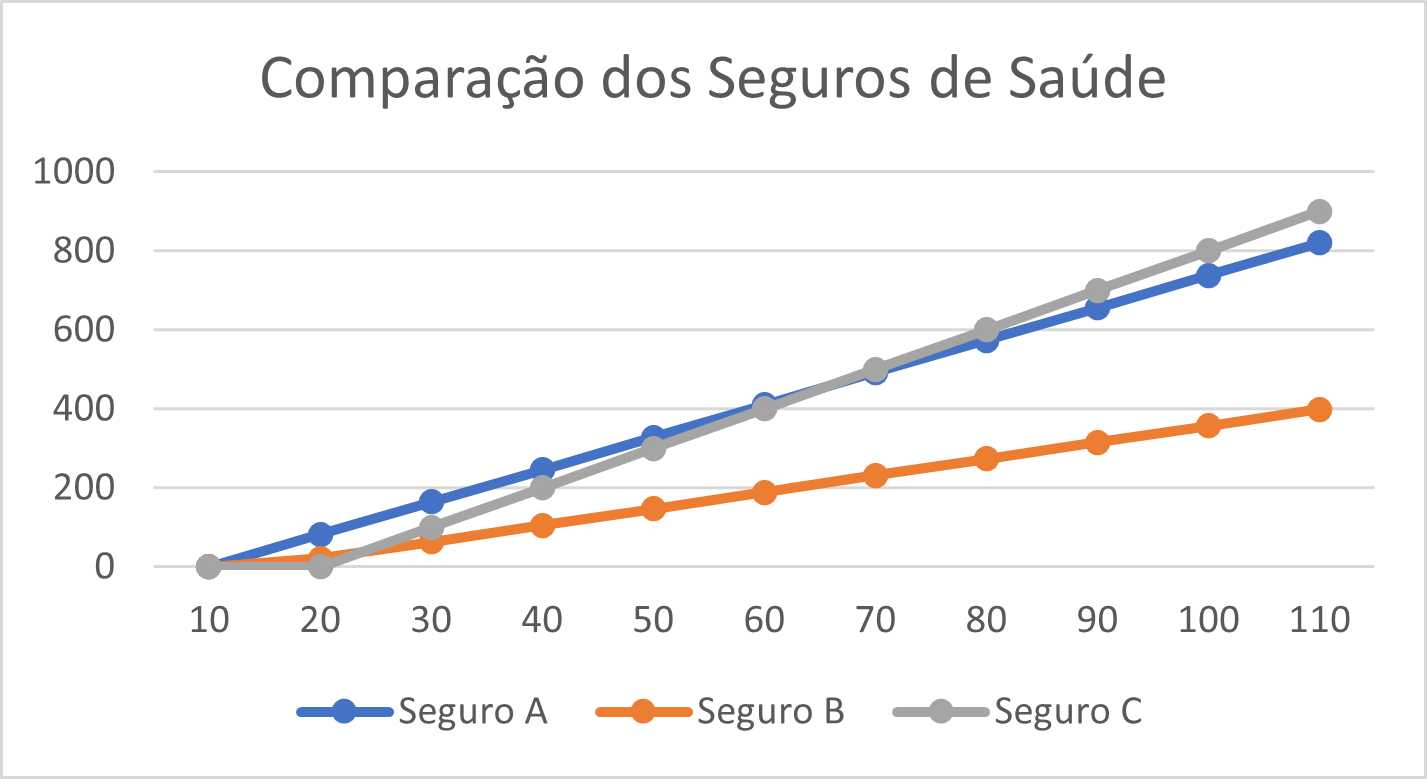
\includegraphics{graph}}

\section{Conclusão}

\newpage

\section{Bibliografia}


\printindex

\end{document}